\section{Proposed Method}
\label{sec:04_method}

\subsection{Overview}
\label{subsec:subsec_41_overview}
Our proposed architecture, BiDecT, leverages backward contextual information for video caption generation. A key distinction from previous bidirectional approaches~\cite{zhongBiTransformerAugmentingSemantic2022, zhongBidirectionalTransformerKnowledge2024} lies in its encoder-free design. Specifically, multimodal features extracted from the input video are projected directly into a bidirectional Transformer decoder without any intermediate encoding stage. This design assumes that representations produced by large-scale pre-trained models are sufficiently informative for direct decoding, making additional encoder-based refinement redundant and computationally costly.

As illustrated in Fig.~\ref{fig:fig04_overall_architecture}, BiDecT represents each input video as a sequence of GOPs rather than densely sampled individual frames, reducing temporal redundancy while preserving local spatio-temporal structure. The overall framework consists of four main components. First, the Multimodal Feature Extraction module derives three complementary modalities—appearance, semantic, and motion—from all GOPs in the video. Second, the Multimodal Feature Embedding module projects these modalities into a shared representation space and combines them into a unified representation. Third, the Backward Decoder (BD) generates a caption in reverse order to construct a global backward context $\MyLVec[1]{H}$. Finally, the Forward Decoder (FD) generates the final caption from left to right while conditioning on both the multimodal representation and $\MyLVec[1]{H}$. The detailed design of each component is presented in the following subsections.

\begin{figure*}[!t]
\centering
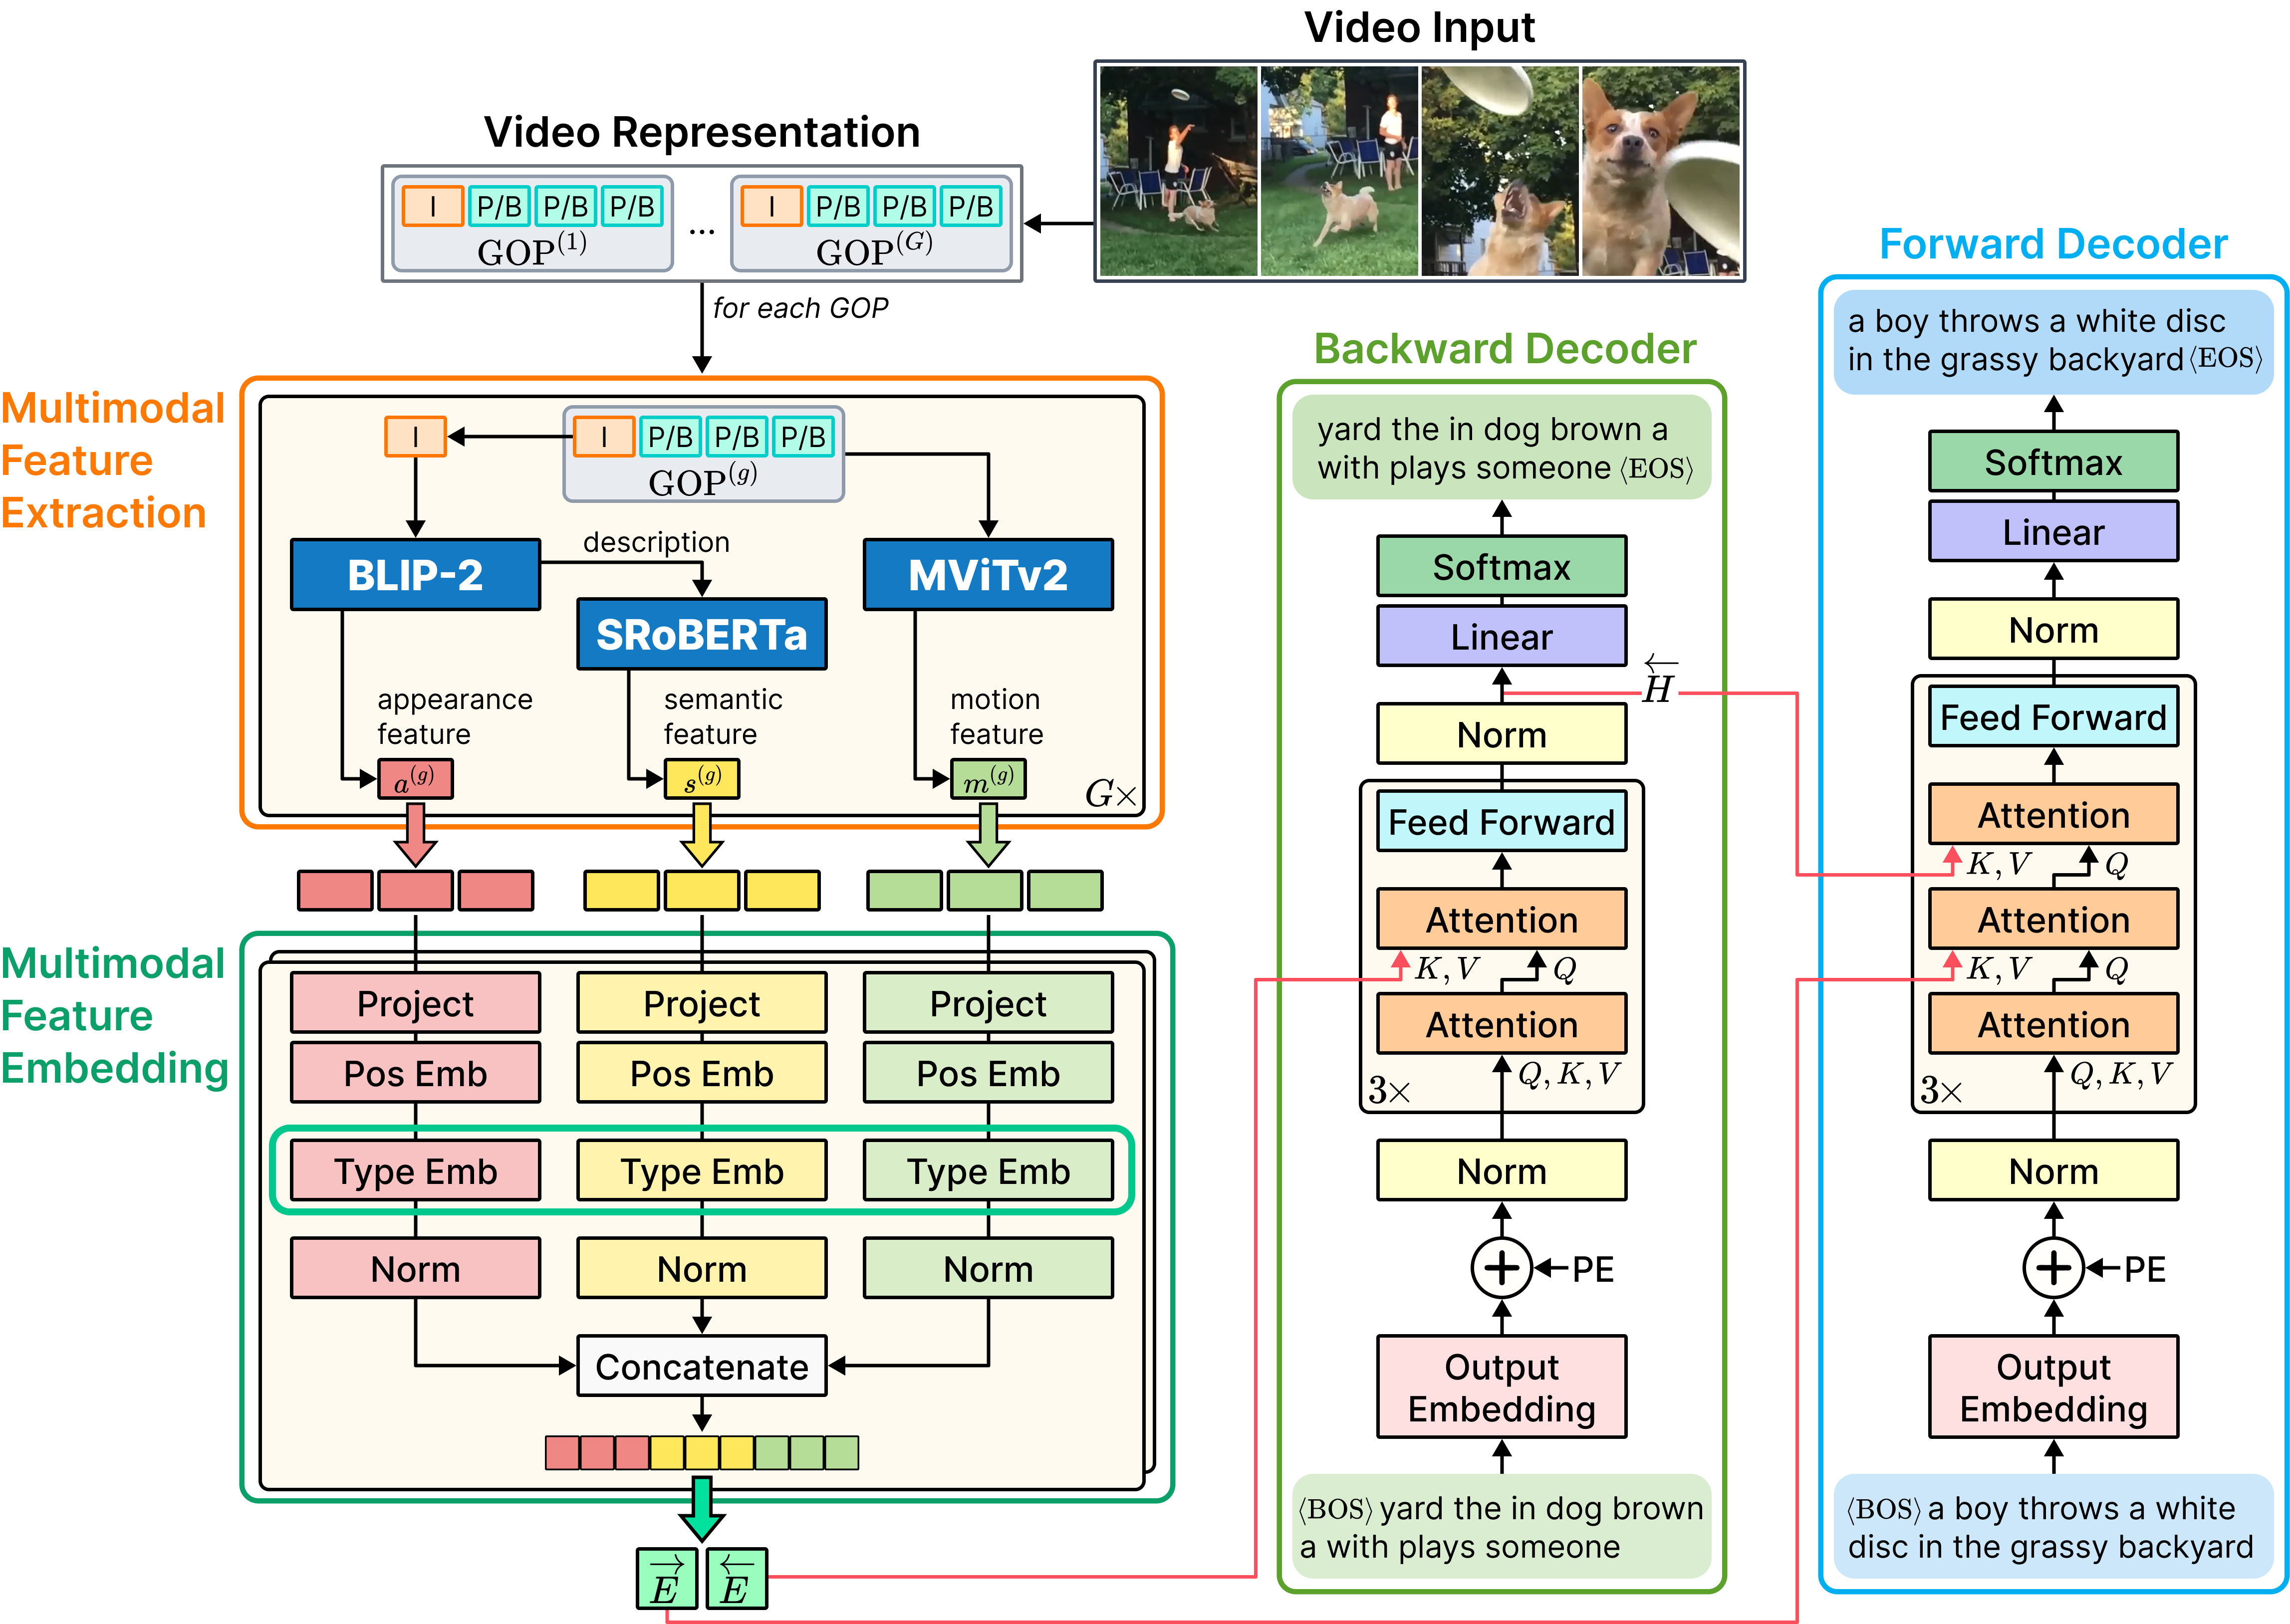
\includegraphics[width=0.90\textwidth, height=8.5in, keepaspectratio]{figures/fig04_overall_architecture.png}
\caption{Overview of the proposed BiDecT architecture. For each GOP, appearance features are extracted using BLIP-2, semantic features are obtained by encoding BLIP-2-generated descriptions with SRoBERTa, and motion features are extracted using MViTv2. These features are projected into a shared representation space and combined into a unified multimodal representation without any intermediate encoding stage. The Backward Decoder (BD) generates a reverse caption to construct a global backward contextual representation $\MyLVec[1]{H}$, while the Forward Decoder (FD) conditions on both the multimodal representation and $\MyLVec[1]{H}$ to generate the final caption.}
\label{fig:fig04_overall_architecture}
\end{figure*}


\subsection{Video Representation and Multimodal Feature Extraction}
\label{subsec:subsec_42_extraction}
Following the GOP representation described earlier, an input video $X$ is formally defined as:
\begin{equation}
X=\left[{\mathrm{GOP}}^{\left(1\right)},\ldots,{\mathrm{GOP}}^{\left(G\right)}\right],
\end{equation}
where $G$ denotes the number of GOPs sampled from the input video. Each GOP begins with an I-frame followed by a sequence of temporally dependent P- and B-frames:
\begin{equation}
{\mathrm{GOP}}^{\left(g\right)}=\left[\mathrm{\operatorname{I}}^{\left(g\right)},{\mathrm{P/\operatorname{B}}}^{\left(g,1\right)},\ldots,{\mathrm{P/\operatorname{B}}}^{\left(g,\mathrm{KeyInt}\texttt{-}1\right)}\right],
\end{equation}
where $\mathrm{KeyInt}$ denotes the Keyframe Interval, i.e., the maximum distance between two consecutive I-frames. Each GOP therefore contains at most $\mathrm{KeyInt}\texttt{-}1$ P/B-frames following the initial I-frame.

For each ${\mathrm{GOP}}^{\left(g\right)}$, BiDecT extracts three complementary modalities from pre-trained models, including appearance, semantic, and motion features. Appearance and motion features capture static scene content and temporal dynamics, respectively, while semantic features bridge low-level visual representations and high-level natural language descriptions.

Since the I-frame provides the most complete spatial representation within each GOP, it serves as the source for both appearance and semantic extraction. The I-frame is processed by the BLIP-2~\cite{liBLIP2BootstrappingLanguageImage2023} image encoder, and the resulting $\mathrm{[CLS]}$ embedding is used as the appearance feature $a^{\left(g\right)}$. The visual representations are also passed to the BLIP-2 caption generator to produce a textual scene description, which is then encoded by SRoBERTa~\cite{reimersSentenceBERTSentenceEmbeddings2019} to obtain the semantic feature $s^{\left(g\right)}$. This dual-purpose extraction strategy transfers visual and linguistic knowledge from image captioning to the video domain without requiring explicit knowledge graph construction.

While the I-frame captures static scene content, it cannot represent the temporal dynamics occurring within the GOP. To model short-term motion information, a frame sequence uniformly sampled from ${\mathrm{GOP}}^{\left(g\right)}$ is processed by MViTv2~\cite{liMViTv2ImprovedMultiscale2022}, producing the motion feature $m^{\left(g\right)}$.

Applying this process across all $G$ GOPs yields three modality-specific feature sequences:

\begin{align}
F_A&=\left[a^{\left(1\right)},\ldots,a^{\left(G\right)}\right]\in\mathbb{R}^{G\times d_A},\\
F_S&=\left[s^{\left(1\right)},\ldots,s^{\left(G\right)}\right]\in\mathbb{R}^{G\times d_S},\\
F_M&=\left[m^{\left(1\right)},\ldots,m^{\left(G\right)}\right]\in\mathbb{R}^{G\times d_M},
\end{align}

% \begin{equation}
% F_A=\left[a^{\left(1\right)},\ldots,a^{\left(G\right)}\right]\in\mathbb{R}^{G\times d_A},
% \end{equation}
% \begin{equation}
% F_S=\left[s^{\left(1\right)},\ldots,s^{\left(G\right)}\right]\in\mathbb{R}^{G\times d_S},
% \end{equation}
% \begin{equation}
% F_M=\left[m^{\left(1\right)},\ldots,m^{\left(G\right)}\right]\in\mathbb{R}^{G\times d_M},
% \end{equation}

where $d_A$, $d_S$, and $d_M$ denote the output dimensions of the corresponding pre-trained models.


\subsection{Multimodal Feature Embedding}
\label{subsec:subsec_43_feat_emb}
The extracted appearance, semantic, and motion features reside in heterogeneous feature spaces of different dimensionalities. Modality-specific linear projections therefore map them into a common $d_{\textit{model}}$-dimensional representation space:
\begin{align}
F_A^\prime&={\mathrm{Linear}}_A(F_A),\\
F_S^\prime&={\mathrm{Linear}}_S(F_S),\\
F_M^\prime&={\mathrm{Linear}}_M(F_M),
\end{align}
where $F_A^\prime,F_S^\prime,F_M^\prime\in\mathbb{R}^{G\times d_{\textit{model}}}$. Using separate projection matrices ensures that each modality undergoes a tailored transformation that accounts for its distinct representational characteristics.

After projection, the three feature sequences cannot be differentiated by the decoder unless their origins are explicitly encoded. Each projected feature is therefore augmented with a learnable type embedding \mbox{$\left(\mathrm{TE}\in\mathbb{R}^{d_{\textit{model}}}\right)$} indicating its source modality, and a shared sinusoidal positional embedding \mbox{$\left(\mathrm{PE}\in\mathbb{R}^{G\times d_{\textit{model}}}\right)$} is added to encode the temporal order of GOPs across all modalities. Modality-specific normalization layers are then applied to stabilize feature magnitudes:
\begin{align}
E_A&={\mathrm{Norm}}_A(F_A^\prime+{\mathrm{TE}}_A+\mathrm{PE}),\\
E_S&={\mathrm{Norm}}_S(F_S^\prime+{\mathrm{TE}}_S+\mathrm{PE}),\\
E_M&={\mathrm{Norm}}_M(F_M^\prime+{\mathrm{TE}}_M+\mathrm{PE}).
\end{align}

The three normalized embeddings are concatenated to form a unified multimodal representation:
\begin{equation}
E=\mathrm{Concat}(E_A,E_S,E_M)\in\mathbb{R}^{3G\times d_{\textit{model}}}.
\end{equation}
This representation maintains temporal correspondence across modalities while preserving modality identity through the type embeddings, enabling the decoder to integrate information from different modalities as needed. The embedding module is instantiated twice with independent parameters, producing $\MyLVec[1]{E}$ and $\MyRVec[1]{E}$ for the backward and forward decoders, respectively, as the two generation directions may require different feature emphasis patterns.


\subsection{Backward Decoder}
\label{subsec:subsec_44_bd}
The Backward Decoder (BD) follows the standard Transformer decoder architecture with Peri-LN applied uniformly across all sub-layers. Unlike conventional left-to-right generation, the BD generates captions in reverse order by conditioning on previously generated reverse tokens together with the multimodal representation $\MyLVec[1]{E}$.

Let $\MyLVec[1]{Z_{t;l}}$ denote the hidden state at decoding step $t$ produced by the $l$-th decoder layer, and let $\MyLVec[1]{Z_{<t;l}}$ denote the hidden states of all preceding positions at the same layer. Each BD layer applies three sequential sub-layers:
\begin{align}
\MyLVec[1]{U_{t;l}} &= \mathrm{MaskedSelfAttn}\Big( \MyLVec[1]{Z_{t;l\texttt{-}1}},\MyLVec[1]{Z_{<t;l\texttt{-}1}},\MyLVec[1]{Z_{<t;l\texttt{-}1}} \Big), \\
\MyLVec[1]{C_{t;l}} &= \mathrm{CrossAttn} \Big( \MyLVec[1]{U_{t;l}},\MyLVec[1]{E},\MyLVec[1]{E} \Big), \\
\MyLVec[1]{Z_{t;l}} &= \mathrm{FFN} \Big( \MyLVec[1]{C_{t;l}} \Big).
\end{align}

The causal mask in masked self-attention ensures that position $t$ attends only to positions $(1,\ldots,t\texttt{-}1)$. The BD comprises $N_{\textit{BD}}$ stacked decoder layers. The hidden state from the final layer is normalized to obtain the per-step backward hidden representation:
\begin{equation}
\MyLVec[1]{h_{t}} = \mathrm{Norm}\Big( \MyLVec[1]{Z_{t;N_{\textit{BD}}}} \Big).
\end{equation}

The probability distribution over the vocabulary at step $t$ is then computed as:
\begin{equation}
P\Big(\MyLVec[1]{y_{t}} \;|\, \MyLVec[1]{Y_{<t}}, \MyLVec[1]{E}\Big) = \mathrm{Softmax}\big( \mathrm{Linear} (\MyLVec[1]{h_{t}}) \big).
\end{equation}

Decoding proceeds autoregressively until the end-of-sequence token \mbox{$\langle \mathrm{EOS} \rangle$} is predicted, yielding the complete reverse caption $\MyLVec[1]{Y} = [\MyLVec[1]{y_{1}},\ldots,\MyLVec[1]{y_{T^\prime}}]$.

Beyond generating the reverse caption, the BD produces a sequence of hidden states encoding a right-to-left semantic representation, collectively forming the global backward context \mbox{$\MyLVec[1]{H} = [\MyLVec[1]{h_{1}},\ldots,\MyLVec[1]{h_{T^\prime}}] \in\mathbb{R}^{T^\prime \times d_{\textit{model}}}$}. This contextual representation is subsequently passed to the Forward Decoder as an auxiliary conditioning signal. Crucially, $\MyLVec[1]{H}$ is not a static encoded representation, but a dynamically generated contextual sequence derived from reverse caption generation. Its quality therefore depends on how effectively the BD learns semantically coherent reverse captions during joint optimization with the Forward Decoder.


\subsection{Forward Decoder}
\label{subsec:subsec_45_fd}
The Forward Decoder (FD) follows the same Transformer decoder architecture as the BD but introduces an additional cross-attention sub-layer for integrating the global backward context. The FD generates the final caption autoregressively from left to right, conditioning on previously generated forward tokens, the multimodal representation $\MyRVec[1]{E}$, and the global backward context $\MyLVec[1]{H}$ produced by the BD.

Let $\MyRVec[1]{Z_{t;l}}$ denote the hidden state at decoding step $t$ produced by the $l$-th decoder layer, and let $\MyRVec[1]{Z_{<t;l}}$ denote the hidden states of all preceding positions at the same layer. Each FD layer applies four sequential sub-layers:
\begin{align}
\MyRVec[1]{U_{t;l}} &= \mathrm{MaskedSelfAttn}\Big( \MyRVec[1]{Z_{t;l\texttt{-}1}},\MyRVec[1]{Z_{<t;l\texttt{-}1}},\MyRVec[1]{Z_{<t;l\texttt{-}1}} \Big), \\
\MyRVec[1]{C_{t;l}} &= \mathrm{CrossAttn}_{E} \Big( \MyRVec[1]{U_{t;l}},\MyRVec[1]{E},\MyRVec[1]{E} \Big), \\
\MyRVec[1]{B_{t;l}} &= \mathrm{CrossAttn}_{H} \Big( \MyRVec[1]{C_{t;l}},\MyLVec[1]{H},\MyLVec[1]{H} \Big), \\
\MyRVec[1]{Z_{t;l}} &= \mathrm{FFN} \Big( \MyRVec[1]{B_{t;l}} \Big).
\end{align}

The additional $\mathrm{CrossAttn}_{H}$ sub-layer enables the FD to attend to the global backward context $\MyLVec[1]{H}$, incorporating right-to-left semantic information that supplements the limited future context available in strictly left-to-right decoding. At inference time, the BD first generates the complete reverse caption to produce $\MyLVec[1]{H}$, after which the FD conditions on this fixed contextual representation to generate the final caption, thereby avoiding direct future-token exposure during forward decoding.

The FD comprises $N_{\textit{FD}}$ stacked decoder layers. The hidden state from the final layer is normalized and then used to compute the probability distribution over the vocabulary at decoding step $t$:
\begin{equation}
\MyRVec[1]{h_{t}} = \mathrm{Norm}\Big( \MyRVec[1]{Z_{t;N_{\textit{FD}}}} \Big),
\end{equation}
\begin{equation}
P\Big(\MyRVec[1]{y_{t}} \;|\, \MyRVec[1]{Y_{<t}},\MyRVec[1]{E},\MyLVec[1]{H} \Big) = \mathrm{Softmax}\big( \mathrm{Linear} (\MyRVec[1]{h_{t}} ) \big).
\end{equation}

Decoding proceeds autoregressively until the end-of-sequence token \mbox{$\langle \mathrm{EOS} \rangle$} is predicted, yielding the final caption $\MyRVec[1]{Y} = [\MyRVec[1]{y_{1}},\ldots,\MyRVec[1]{y_{T}}]$.


\subsection{Optimization}
\label{subsec:subsec_46_optim}
BiDecT is trained by jointly optimizing the backward and forward decoders using cross-entropy objectives. For a given video $X$ with multimodal embeddings $\MyLVec[1]{E}$ and $\MyRVec[1]{E}$, let \mbox{$\MyRVec[1]{Y} = [\MyRVec[1]{y_{1}},\ldots,\MyRVec[1]{y_{L}}]$} denote the ground-truth forward caption, and let \mbox{$\MyLVec[1]{Y} = [\MyLVec[1]{y_{1}},\ldots,\MyLVec[1]{y_{L^\prime}}]$} denote the corresponding pseudo reverse caption. The backward and forward decoding objectives are defined as:
\begin{align}
\mathcal{L}_{\textit{BD}} &= - \sum_{t=1}^{L^\prime} \mathrm{log}\; P\Big(\MyLVec[1]{y_{t}} \;|\, \MyLVec[1]{Y_{<t}}, \MyLVec[1]{E}; \, \theta_{\textit{BD}} \Big),
\\
\mathcal{L}_{\textit{FD}} &= - \sum_{t=1}^{L} \mathrm{log}\; P\Big(\MyRVec[1]{y_{t}} \;|\, \MyRVec[1]{Y_{<t}},\MyRVec[1]{E},\MyLVec[1]{H}; \, \theta_{\textit{BD}},\theta_{\textit{FD}} \Big),
\end{align}
where $\theta_{\textit{BD}}$ and $\theta_{\textit{FD}}$ denote the trainable parameters of the backward and forward decoders, respectively. Importantly, $\mathcal{L}_{\textit{FD}}$ explicitly depends on $\theta_{\textit{BD}}$ because the FD conditions on the global backward context $\MyLVec[1]{H}$ generated by the BD. Gradients from $\mathcal{L}_{\textit{FD}}$ therefore propagate through the BD, allowing $\MyLVec[1]{H}$ to be jointly optimized for both reverse and forward caption generation.

The overall training objective combines both terms:
\begin{equation}
\mathcal{L}=(1\texttt{-}\lambda)\,\mathcal{L}_{\textit{BD}}+\lambda\,\mathcal{L}_{\textit{FD}},
\end{equation}
where \mbox{$\lambda \in [0,1]$} controls the relative contribution of the backward and forward decoding objectives.

\begin{figure}[!t]
\centering
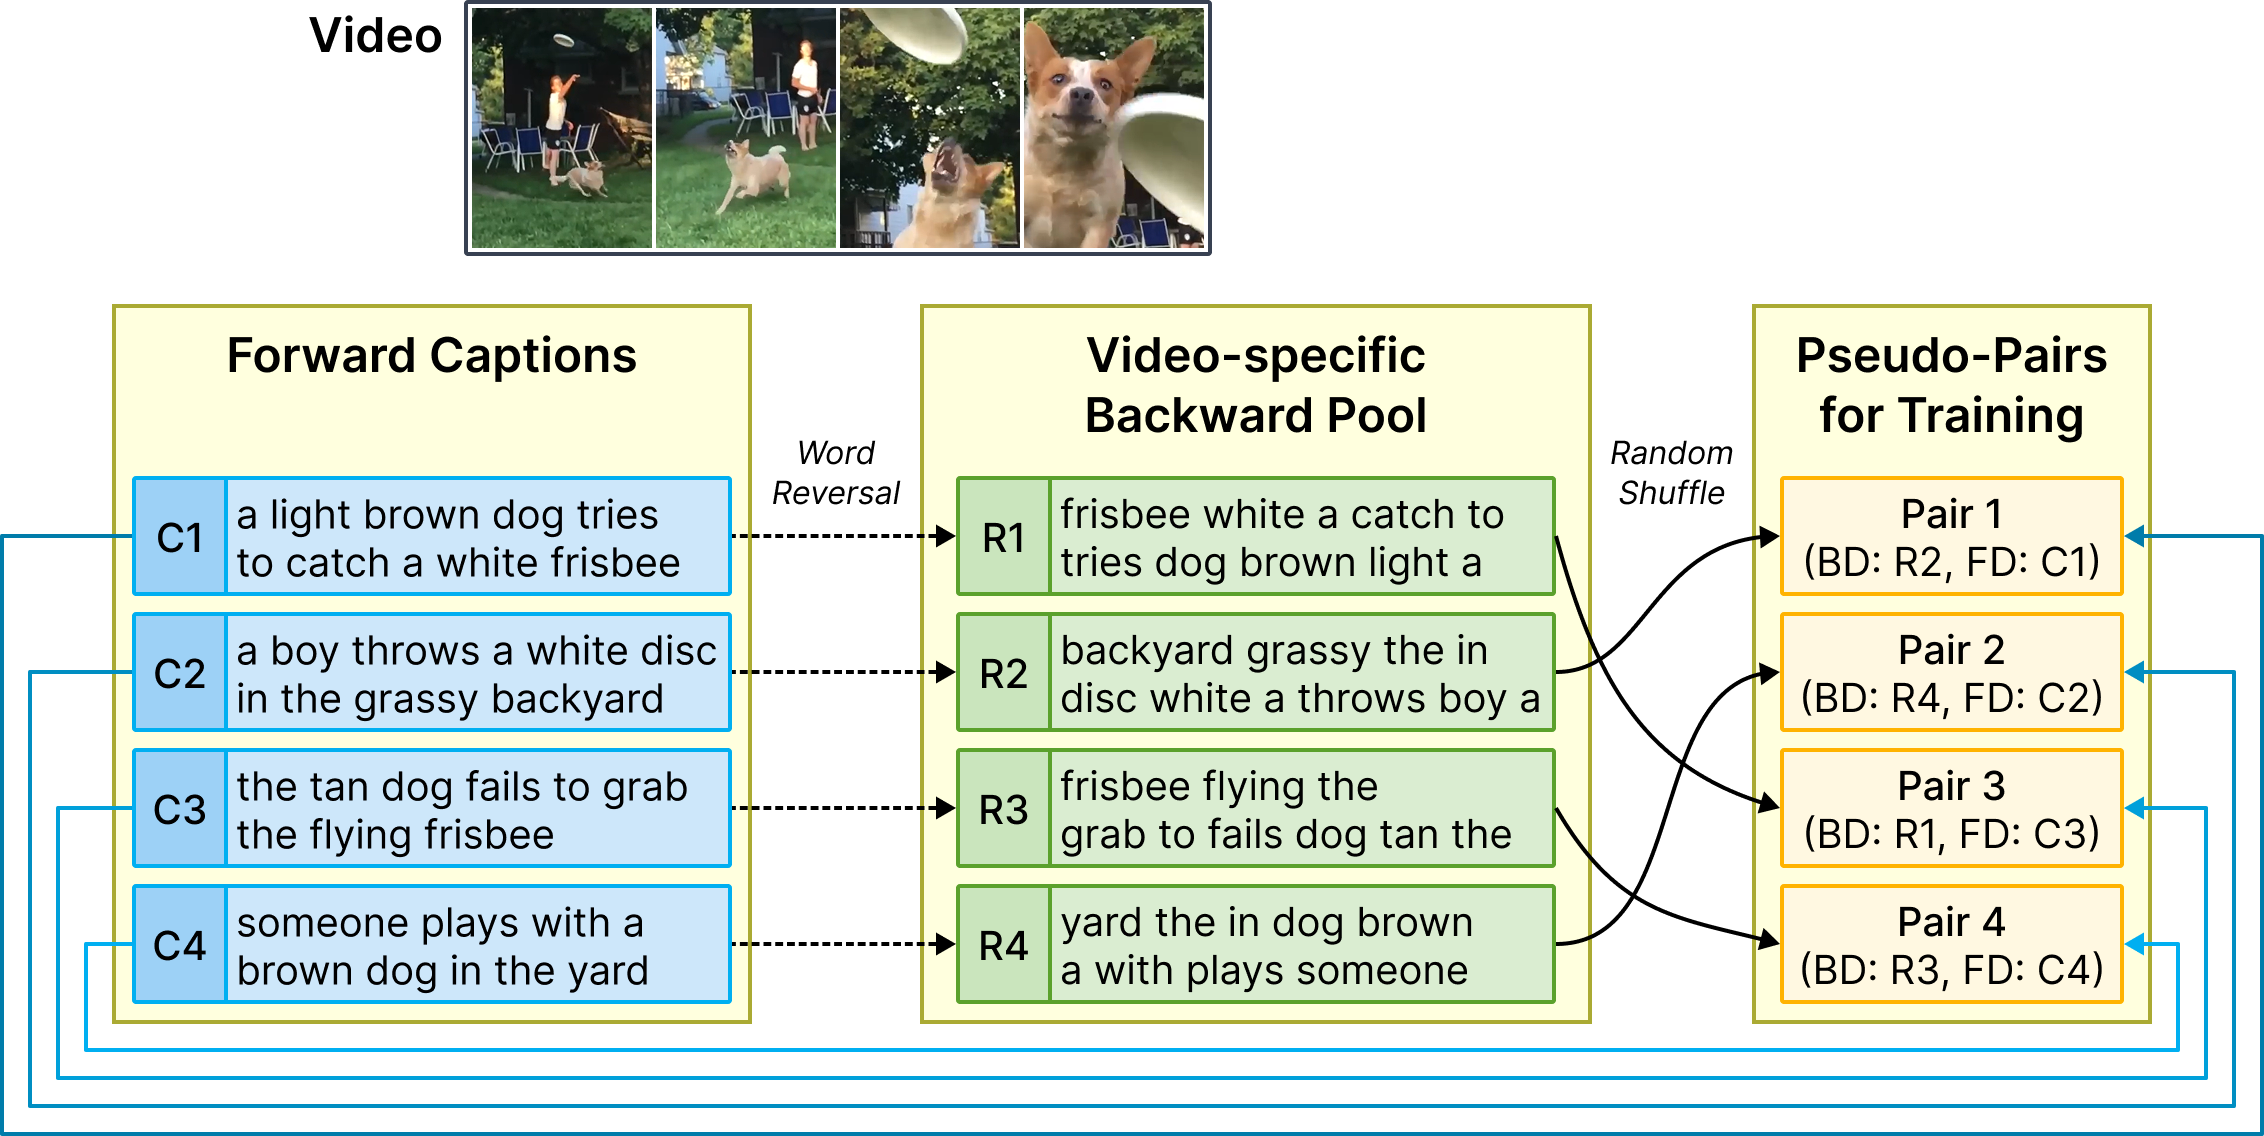
\includegraphics[width=0.99\columnwidth]{figures/fig05_pseudo_reverse_captions.png}
\caption{Construction of pseudo reverse captions for bidirectional training. Forward captions from the same video are reversed, shuffled, and pseudo-paired with different forward captions to prevent direct token-level correspondence between $\MyLVec[1]{H}$ and the target forward caption.}
\label{fig:fig05_pseudo_reverse_captions}
\end{figure}

A central challenge in training bidirectional decoders is preventing information leakage between the two decoding directions. If the BD were supervised using the exact reversed sequence of the target forward caption, the FD could trivially exploit the token-level correspondence implicitly encoded in $\MyLVec[1]{H}$, effectively learning to copy future tokens rather than generate captions grounded in the multimodal input. At inference time, this shortcut becomes unavailable because the BD must generate reverse captions without access to ground-truth targets, leading to poor generalization during inference.

To address this issue, we adopt a pseudo reverse caption strategy following prior bidirectional decoding approaches~\cite{zhongBiTransformerAugmentingSemantic2022, zhongBidirectionalTransformerKnowledge2024}. As illustrated in Fig.~\ref{fig:fig05_pseudo_reverse_captions}, all forward captions associated with the same video are first reversed to form a video-specific backward pool. These reversed captions are then randomly shuffled and pseudo-paired with different forward captions from the same video. Because all pseudo reverse captions originate from the same video, the backward context remains semantically aligned with the visual content while avoiding direct token-level correspondence with any specific target caption. Consequently, the resulting $\MyLVec[1]{H}$ encodes meaningful right-to-left semantic structure that the FD can exploit to generate more coherent and visually grounded captions.


\subsection{Complexity Analysis}
\label{subsec:subsec_47_complexity}
This section analyzes how the computational complexity of encoder-based and encoder-free bidirectional decoder architectures scales with $G$, the number of GOPs representing an input video. Let $d_{\textit{model}}$ denote the model dimension, and let $L$ and $L^\prime$ denote the lengths of the forward and backward captions, respectively. Since multimodal feature extraction is performed offline prior to training, the analysis focuses on how the complexity of each architecture scales with $G$. The multimodal embedding module introduces only linear complexity in $G$ and is common to both architectures, so it does not affect the asymptotic comparison.

In encoder-based architectures, multimodal tokens are processed by Transformer encoder layers before decoding. Self-attention over a sequence of length proportional to $G$ incurs quadratic complexity, while the FFN contributes linearly, yielding an encoding stage complexity of:
\begin{equation}
\mathcal{O}\left(G^2\cdot d_{\textit{model}}+G\cdot d_{\textit{model}}^2\right).
\end{equation}

In both architectures, the decoder accesses the multimodal sequence through cross-attention. The only $G$-dependent cost at the decoding stage is cross-attention to the multimodal representation in both the BD and FD, yielding a combined complexity of:
\begin{equation}
\mathcal{O}\left((L+L^\prime)\cdot G\cdot d_{\textit{model}}\right).
\end{equation}
All remaining decoder components depend only on caption lengths $L$ and $L^\prime$, which are typically much smaller than $G$.

Encoder-based architectures therefore incur both the quadratic encoding cost and the linear decoding cost, with the quadratic term dominating as $G$ increases. By eliminating the encoding stage, BiDecT reduces the dominant computational complexity from quadratic to linear in $G$, an advantage that becomes increasingly significant for long videos with large numbers of GOPs.

% ==== TODO: Complexity Analysis Summary Table ====
% Table~\ref{tab:complexity} summarizes the $G$-dependent terms, and the practical impact of this reduction is empirically validated in Section~\ref{subsec:subsec_54_main_results}.

% \begin{table}[!t]
% \caption{Computational complexity comparison between encoder-based and encoder-free bidirectional decoder architectures as a function of the number of GOPs $G$.}
% \label{tab:complexity}
% \centering
% \begin{tabular}{l c c}
% \hline\hline
% \textbf{Component} & \textbf{Encoder-based} & \textbf{Encoder-free (BiDecT)} \\
% \hline
% Encoding stage & $\mathcal{O}(G^2 \cdot d_{\textit{model}})$ & --- \\
% Decoding stage & \multicolumn{2}{c}{$\mathcal{O}((L+L^\prime) \cdot G \cdot d_{\textit{model}})$} \\
% Dominant scaling in $G$ & Quadratic $\mathcal{O}(G^2)$ & Linear $\mathcal{O}(G)$ \\
% \hline\hline
% \end{tabular}
% \end{table}


